% !TeX program = lualatex
\documentclass[11pt, aspectratio=169]{beamer}
\usepackage[utf8]{inputenc}
\usepackage[T1]{fontenc}
\usepackage{amsmath, amssymb, bm}
\usepackage{booktabs, array, multirow, colortbl}
\usepackage{graphicx}
\usepackage{xcolor}
\usepackage{tikz}
\usepackage{pgfplots}
\pgfplotsset{compat=1.18}
\usetikzlibrary{shapes.geometric, arrows.meta, positioning, calc, trees, fit, backgrounds}
\usepackage{listings}
\usepackage{hyperref}
\usepackage{tcolorbox}
\tcbuselibrary{skins, breakable}

% ─── Theme & Palette ────────────────────────────────────────────────────────
\usetheme{Madrid}
\usecolortheme{default}

% Light palette — soft blues / teals on near-white
\definecolor{navyblue}{RGB}{30, 80, 140}
\definecolor{oceanblue}{RGB}{42, 130, 210}
\definecolor{skyblue}{RGB}{100, 185, 255}
\definecolor{tealgreen}{RGB}{0, 150, 170}
\definecolor{emerald}{RGB}{67, 160, 71}
\definecolor{amber}{RGB}{249, 168, 37}
\definecolor{alertred}{RGB}{200, 50, 50}
% Code block: light background, dark text  (Courier New feel)
\definecolor{codebg}{RGB}{245, 247, 250}
\definecolor{codefg}{RGB}{30,  40,  60}
\definecolor{codekw}{RGB}{0,   80, 160}
\definecolor{codecomment}{RGB}{100, 120, 150}
\definecolor{codestring}{RGB}{0, 130, 100}
\definecolor{lightgray}{RGB}{235, 240, 248}
\definecolor{midgray}{RGB}{130, 150, 175}
\definecolor{darktext}{RGB}{26, 35, 60}
\definecolor{ugold}{RGB}{249, 168, 37}
\definecolor{frameborder}{RGB}{160, 190, 220}

\setbeamercolor{palette primary}{bg=navyblue, fg=white}
\setbeamercolor{palette secondary}{bg=navyblue!75, fg=white}
\setbeamercolor{palette tertiary}{bg=tealgreen, fg=white}
\setbeamercolor{palette quaternary}{bg=navyblue, fg=white}
\setbeamercolor{structure}{fg=navyblue}
\setbeamercolor{section in toc}{fg=navyblue}
\setbeamercolor{alerted text}{fg=alertred}
\setbeamercolor{block title}{bg=navyblue!85, fg=white}
\setbeamercolor{block body}{bg=lightgray, fg=darktext}
\setbeamercolor{block title alerted}{bg=alertred!85, fg=white}
\setbeamercolor{block body alerted}{bg=alertred!8, fg=darktext}
\setbeamercolor{block title example}{bg=tealgreen!85, fg=white}
\setbeamercolor{block body example}{bg=tealgreen!8, fg=darktext}
\setbeamercolor{background canvas}{bg=white}
\setbeamercolor{normal text}{fg=darktext}

% ─── tcolorbox exercise environment ──────────────────────────────────────────
\tcbset{
	exercisestyle/.style={
		enhanced, breakable,
		colback=navyblue!5, colframe=navyblue!60,
		fonttitle=\bfseries\small,
		title={Exercise},
		attach boxed title to top left={yshift=-2mm, xshift=4mm},
		boxed title style={colback=navyblue!80, colframe=navyblue!80},
		left=4pt, right=4pt, top=4pt, bottom=4pt
	}
}
\newtcolorbox{exercise}[1][]{exercisestyle, title={#1}}

% ─── Code listing style — Courier New look on light background ───────────────
\lstdefinestyle{Rstyle}{
	language=R,
	basicstyle=\fontfamily{pcr}\selectfont\scriptsize\color{codefg},
	keywordstyle=\fontfamily{pcr}\selectfont\bfseries\color{codekw},
	commentstyle=\fontfamily{pcr}\selectfont\itshape\color{codecomment},
	stringstyle=\fontfamily{pcr}\selectfont\color{codestring},
	backgroundcolor=\color{codebg},
	frame=single,
	framerule=0.5pt,
	rulecolor=\color{frameborder},
	breaklines=true,
	showstringspaces=false,
	tabsize=2,
	numbers=none,
	xleftmargin=5pt,
	xrightmargin=5pt,
	aboveskip=4pt,
	belowskip=2pt
}
\lstset{style=Rstyle}

% ─── Footline ────────────────────────────────────────────────────────────────
\setbeamertemplate{navigation symbols}{}
\setbeamertemplate{footline}{%
	\leavevmode
	\hbox{%
		\begin{beamercolorbox}[wd=.35\paperwidth,ht=2.25ex,dp=1ex,left,leftskip=4pt]{palette primary}
			\usebeamerfont{author in head/foot}R.\ Minkah --- Dept.\ of Statistics \& Actuarial Science
		\end{beamercolorbox}%
		\begin{beamercolorbox}[wd=.40\paperwidth,ht=2.25ex,dp=1ex,center]{palette secondary}
			\usebeamerfont{title in head/foot}BDAT 608: Computational Statistics in Big Data II
		\end{beamercolorbox}%
		\begin{beamercolorbox}[wd=.25\paperwidth,ht=2.25ex,dp=1ex,right,rightskip=4pt]{palette primary}
			\usebeamerfont{date in head/foot}%
			University of Ghana\hspace{1em}\insertframenumber{}/\inserttotalframenumber
		\end{beamercolorbox}%
	}%
}

% ─── Metadata ────────────────────────────────────────────────────────────────
\title[Regression with sparklyr]{%
	Regression Modelling\\[4pt]
	with \texttt{sparklyr} and Apache Spark MLlib}
\subtitle{Simple Linear $\cdot$ Multiple Linear $\cdot$ Logistic Regression}
\author[R.\ Minkah]{Richard Minkah, PhD}
\institute[Dept.\ Statistics \& Actuarial Sci.]{%
	Department of Statistics \& Actuarial Science\\
	University of Ghana, Legon\\[2pt]
	\textit{Mastering Spark with R / therinspark.com} --- Chapter 4 (Luraschi, Kuo \& Ushey, 2019)}
\date{BDAT 608 --- \today}

% ─── Helper commands ────────────────────────────────────────────────────────
\newcommand{\Rfun}[1]{\texttt{\textcolor{codekw}{#1}}}
\newcommand{\Rpkg}[1]{\texttt{\textcolor{tealgreen}{#1}}}

\begin{document}

% ─────────────────────────────────────────────────────────────────────────────
% TITLE SLIDE
% ─────────────────────────────────────────────────────────────────────────────
{
	\setbeamertemplate{footline}{}
	\begin{frame}[plain]
		\begin{tikzpicture}[remember picture, overlay]
			% Background
			\fill[navyblue!10] (current page.south west) rectangle (current page.north east);
			\fill[navyblue!20] ([xshift=8.5cm]current page.south west)
			rectangle (current page.north east);
			\fill[tealgreen!70] ([xshift=8.5cm]current page.south west)
			rectangle ([xshift=8.60cm]current page.north west);
			% Decorative circles
			\fill[oceanblue!40] (12.6,4.5) circle (1.5cm);
			\fill[skyblue!60]   (12.9,4.9) circle (0.8cm);
			\fill[tealgreen!50] (12.2,1.9) circle (1.2cm);
			\fill[navyblue!30]  (12.5,2.2) circle (0.55cm);
			% Banner
			\fill[ugold] (1.0,6.0) rectangle (4.4,6.45);
			\node[navyblue, font=\bfseries\scriptsize] at (2.7,6.22)
			{BDAT 608 --- University of Ghana, Legon};
			\fill[tealgreen!80] (1.0,5.55) rectangle (4.4,5.95);
			\node[white, font=\bfseries\scriptsize] at (2.7,5.75)
			{sparklyr + Apache Spark MLlib};
			% Title text
			\node[navyblue, font=\bfseries\Large, align=left, anchor=west]
			at (1.0,5.10) {Regression Modelling};
			\node[oceanblue, font=\bfseries\Large, align=left, anchor=west]
			at (1.0,4.50) {with \texttt{sparklyr}};
			\node[midgray, font=\small, align=left, anchor=west]
			at (1.0,3.80) {Simple Linear $\cdot$ Multiple Linear $\cdot$ Logistic Regression};
			\draw[tealgreen, line width=1.5pt] (1.0,3.35) -- (5.8,3.35);
			\node[darktext, font=\footnotesize, align=left, anchor=west]
			at (1.0,2.95) {\textbf{Topics:} Model fitting $\cdot$ Parameter interpretation};
			\node[darktext, font=\footnotesize, align=left, anchor=west]
			at (1.0,2.55) {Hypothesis testing $\cdot$ Diagnostics $\cdot$ Model selection};
			\node[darktext, font=\footnotesize, align=left, anchor=west]
			at (1.0,2.15) {OkCupid running example from \texttt{therinspark.com}};
			\node[midgray, font=\itshape\tiny, anchor=west]
			at (1.0,0.6) {Luraschi, Kuo \& Ushey (2019). Mastering Spark with R. O'Reilly.};
		\end{tikzpicture}
	\end{frame}
}

% ─────────────────────────────────────────────────────────────────────────────
% TABLE OF CONTENTS
% ─────────────────────────────────────────────────────────────────────────────
\begin{frame}{Outline}
	\tableofcontents
\end{frame}

% =============================================================================
\section{Setup: Data \& sparklyr Workflow}
% =============================================================================

\begin{frame}[fragile,allowframebreaks]{The OkCupid Dataset \& sparklyr Setup}
	\begin{block}{About the data (therinspark.com Ch.\ 4)}
				\begin{itemize}
					\item $\approx$60\,000 user profiles from OkCupid
					\item Biographical: \texttt{age}, \texttt{sex}, \texttt{height},
					\texttt{job}, \texttt{education}
					\item Behavioural: \texttt{drinks}, \texttt{drugs}, \texttt{smokes}
					\item 10 free-text essay fields (\texttt{essay0}--\texttt{essay9})
				\end{itemize}
				Two response variables used across sections:
				\begin{itemize}
					\item \textbf{Regression:} \texttt{essay\_length} (continuous)
					\item \textbf{Classification:} \texttt{not\_working} (binary 0/1)
				\end{itemize}
			\end{block}
			\begin{alertblock}{Golden rule}
				Always split \emph{before} any scaling or encoding.
				Fit all transformers on the \textbf{training set only}.
			\end{alertblock}
		\begin{lstlisting}[title={Loading, cleaning \& splitting (therinspark.com §4.1--4.2)}]
library(sparklyr); library(dplyr)
sc <- spark_connect(master = "local",
                    version = "2.3")

okc <- spark_read_csv(
  sc, "data/profiles.csv",
  escape  = "\"",
  options = list(multiline = TRUE)) %>%
  mutate(
    essay_length = nchar(paste(
      essay0, essay1, essay2, essay3,
      sep = " ")),
    scaled_age = (age - mean(age)) /
                  sd(age),
    income = ifelse(income == "-1",
             NA_real_, as.numeric(income)),
    not_working = as.integer(
      job %in% c("retired","student",
                 "unemployed"))
  )

splits    <- sdf_random_split(
  okc, training = 0.8, test = 0.2,
  seed = 42)
okc_train <- splits$training
okc_test  <- splits$test
			\end{lstlisting}
		\end{frame}

% =============================================================================
\section{Simple Linear Regression}
% =============================================================================

% ── SLR 1: Model & Assumptions ───────────────────────────────────────────────
\begin{frame}[fragile,allowframebreaks]{Simple Linear Regression --- Model \& Assumptions}
	\begin{block}{The simple linear model}
				For a single predictor $x_i$ and response $y_i$:
				\[
				y_i = \beta_0 + \beta_1 x_i + \varepsilon_i,
				\qquad i = 1,\ldots,n
				\]
				\textbf{OLS estimators} minimise the residual sum of squares:
				\[
				\hat\beta_1 = \frac{\sum(x_i-\bar x)(y_i-\bar y)}{\sum(x_i-\bar x)^2},
				\quad
				\hat\beta_0 = \bar y - \hat\beta_1\bar x
				\]
			\end{block}
			\begin{block}{Gauss--Markov assumptions (CLASS)}
				\begin{enumerate}\footnotesize
					\item \textbf{C}orrect functional form (linearity)
					\item \textbf{L}ack of perfect multicollinearity
					\item \textbf{A}bsence of correlation between $\varepsilon_i$ and $x_i$
					\item \textbf{S}phericity: $\varepsilon_i \overset{\mathrm{iid}}{\sim}(0,\sigma^2)$
					(homoscedasticity + no autocorrelation)
					\item \textbf{S}parse outliers / influential points
				\end{enumerate}
				Under these, OLS is \textbf{BLUE} (Best Linear Unbiased Estimator).
			\end{block}
		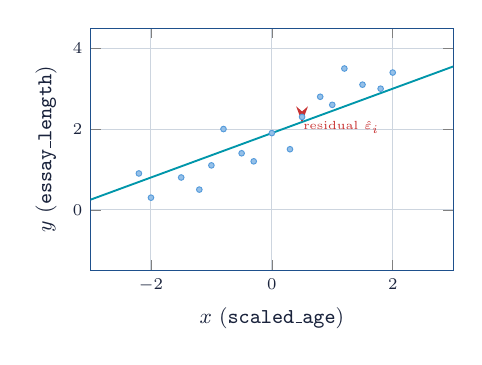
\begin{tikzpicture}[scale=0.85]
				\begin{axis}[
					xlabel={$x$ (\texttt{scaled\_age})},
					ylabel={$y$ (\texttt{essay\_length})},
					xmin=-3, xmax=3, ymin=-1.5, ymax=4.5,
					grid=major, grid style={midgray!40},
					axis line style={navyblue},
					tick label style={font=\scriptsize, color=darktext},
					label style={font=\small, color=darktext},
					width=7cm, height=5.2cm]
					\addplot[only marks, mark=*, mark size=1.2pt,
					mark options={fill=oceanblue!50, draw=oceanblue!80}]
					coordinates {
						(-2,0.3)(-1.5,0.8)(-1,1.1)(-0.5,1.4)(0,1.9)(0.5,2.3)
						(1,2.6)(1.5,3.1)(2,3.4)(-2.2,0.9)(-0.8,2.0)(0.3,1.5)
						(1.2,3.5)(-1.2,0.5)(0.8,2.8)(-0.3,1.2)(1.8,3.0)
					};
					\addplot[tealgreen, thick, domain=-3:3]{0.55*x + 1.9};
					\draw[alertred, -Stealth, thick]
					(axis cs:0.5, 2.2) -- (axis cs:0.5, 2.175);
					\node[alertred, font=\tiny] at (axis cs:1.15,2.05)
					{residual $\hat\varepsilon_i$};
				\end{axis}
			\end{tikzpicture}
			\begin{lstlisting}[title={SLR in sparklyr (therinspark.com)}]
slr <- ml_linear_regression(
  okc_train,
  essay_length ~ scaled_age)

summary(slr)
# Coefficients:
#   (Intercept)  2148.3
#   scaled_age    312.1
# RMSE: 1847.2   R^2: 0.041
			\end{lstlisting}
		\end{frame}

% ── SLR 2: Parameter Interpretation ─────────────────────────────────────────
\begin{frame}[fragile,allowframebreaks]{Simple Linear Regression --- Parameter Interpretation}
	\begin{block}{Interpreting $\hat\beta_0$ and $\hat\beta_1$}
				\begin{itemize}
					\item $\hat\beta_0 = 2148.3$: predicted \texttt{essay\_length} when
					\texttt{scaled\_age} $= 0$ (i.e.\ at the mean age).
					\item $\hat\beta_1 = 312.1$: for each one standard-deviation
					increase in age, expected essay length increases by
					$\approx 312$ characters.
					\item Since \texttt{scaled\_age} $= (age - \bar{age})/\widehat{sd}$,
					a one-year increase in age corresponds to
					$312.1 / \widehat{sd}$ more characters.
				\end{itemize}
			\end{block}
			\begin{block}{Coefficient of determination}
				\[
				R^2 = 1 - \frac{\mathrm{SSE}}{\mathrm{SST}} = 0.041
				\]
				Age alone explains only 4.1\% of the variation in essay
				length --- motivating the multiple regression model.
			\end{block}
		\begin{lstlisting}[title={Extracting coefficients \& R² (therinspark.com)}]
s <- summary(slr)

# Coefficient table
s$coefficients
#        features  Estimate  Std. Error
# (Intercept)      2148.26    11.22
# scaled_age        312.07    14.80

# Fit statistics
s$r.squared                  # 0.041
s$root_mean_squared_error    # 1847.2

# Fitted values
preds <- ml_predict(slr, okc_test)
preds %>%
  select(essay_length, prediction) %>%
  head(5) %>% collect()
# essay_length  prediction
#         3241      2614.2
#          892      1987.4
			\end{lstlisting}
			\begin{exampleblock}{Interpretation rule}
				Always state the units of both $x$ and $y$ when reporting
				slope coefficients.  For standardised predictors, the
				natural unit is ``per standard deviation.''
			\end{exampleblock}
		\end{frame}

% ── SLR 3: Hypothesis Testing ────────────────────────────────────────────────
\begin{frame}[fragile,allowframebreaks]{Simple Linear Regression --- Hypothesis Tests}
	\begin{block}{Test for slope: $H_0: \beta_1 = 0$}
				\[
				t = \frac{\hat\beta_1}{\mathrm{SE}(\hat\beta_1)}
				= \frac{312.1}{14.8} \approx 21.1
				\sim t_{n-2} \quad\text{under }H_0
				\]
				$p \ll 0.001$: strong evidence that age is a significant
				predictor of essay length.
			\end{block}
			\begin{block}{95\% Confidence interval for $\beta_1$}
				\[
				\hat\beta_1 \pm t_{n-2,\,0.025}\cdot\mathrm{SE}(\hat\beta_1)
				\approx 312.1 \pm 1.96 \times 14.8
				= [283.1,\; 341.1]
				\]
			\end{block}
			\begin{block}{Overall $F$-test (same as $t^2$ for SLR)}
				\[
				F = t^2 \approx 21.1^2 = 445.2 \sim F_{1,\,n-2}
				\]
				Equivalent to $H_0: \beta_1 = 0$ in the SLR case.
			\end{block}
		\begin{lstlisting}[title={t-test via GLM (gives p-values directly)}]
# ml_generalized_linear_regression
# returns std. errors and p-values
glm_slr <- ml_generalized_linear_regression(
  okc_train,
  essay_length ~ scaled_age,
  family = "gaussian",
  link   = "identity")

library(broom)
tidy(glm_slr)
# term         estimate std.error statistic  p.value
# (Intercept)  2148.26    11.22    191.5   < 2e-16
# scaled_age    312.07    14.80     21.1   < 2e-16

confint(glm_slr)
#              2.5 %   97.5 %
# (Intercept) 2126.3   2170.3
# scaled_age   283.1    341.1
			\end{lstlisting}
			\begin{alertblock}{Note on sparklyr}
				\Rfun{ml\_linear\_regression()} returns standard errors
				but \emph{not} $p$-values.  Use
				\Rfun{ml\_generalized\_linear\_regression()} with
				\texttt{family = "gaussian"} for full inference output.
			\end{alertblock}
		\end{frame}

% ── SLR 4: Diagnostics ───────────────────────────────────────────────────────
\begin{frame}[fragile,allowframebreaks]{Simple Linear Regression --- Diagnostics}
	\begin{block}{Residual diagnostic plots}
				\begin{itemize}
					\item \textbf{Residuals vs.\ Fitted}: should scatter randomly
					around zero --- checks linearity \& homoscedasticity
					\item \textbf{Normal Q--Q}: points near the diagonal confirm
					normality of residuals
					\item \textbf{Scale--Location}: $\sqrt{|\hat\varepsilon_i|}$ vs $\hat y_i$
					--- flat loess confirms constant variance
					\item \textbf{Cook's distance / Leverage}: identifies high-influence
					observations
				\end{itemize}
			\end{block}
			\begin{lstlisting}[title={Extract residuals in sparklyr}]
preds_tr <- ml_predict(slr, okc_train) %>%
  mutate(
    residual  = essay_length - prediction,
    std_resid = residual /
      summary(slr)$root_mean_squared_error
  )

resid_df <- preds_tr %>%
  select(prediction, residual, std_resid,
         scaled_age) %>%
  sample_frac(0.05) %>% collect()
			\end{lstlisting}
		\begin{lstlisting}[title={Residuals vs Fitted}]
library(ggplot2)
ggplot(resid_df,
       aes(x = prediction, y = residual)) +
  geom_point(alpha = 0.3,
             color = "steelblue", size = 0.8) +
  geom_hline(yintercept = 0,
             linetype = "dashed",
             color = "red") +
  geom_smooth(method = "loess", se = FALSE,
              color = "darkred",
              linewidth = 0.8) +
  labs(title = "Residuals vs Fitted (SLR)",
       x = "Fitted values",
       y = "Residuals") +
  theme_minimal()
			\end{lstlisting}
			\begin{lstlisting}[title={Normal Q--Q plot}]
ggplot(resid_df,
       aes(sample = std_resid)) +
  stat_qq(color = "steelblue", size = 0.7) +
  stat_qq_line(color = "red",
               linetype = "dashed") +
  labs(title = "Normal Q-Q (SLR)",
       x = "Theoretical quantiles",
       y = "Standardised residuals") +
  theme_minimal()
			\end{lstlisting}
			\begin{exercise}[Exercise]
				Using a 5\% sample of residuals, construct a scale--location
				plot for the SLR and comment on whether the homoscedasticity
				assumption appears satisfied.
			\end{exercise}
		\end{frame}

% =============================================================================
\section{Multiple Linear Regression}
% =============================================================================

% ── MLR 1: Model & Matrix Form ───────────────────────────────────────────────
\begin{frame}[fragile,allowframebreaks]{Multiple Linear Regression --- Model \& Matrix Form}
	\begin{block}{From SLR to MLR}
				With $p$ predictors $x_1,\ldots,x_p$:
				\[
				y_i = \beta_0 + \beta_1 x_{i1} + \cdots + \beta_p x_{ip}
				+ \varepsilon_i
				\]
				In matrix notation:
				$\mathbf{X} \in \mathbb{R}^{n\times(p+1)}$:
				\[
				\mathbf{y} = \mathbf{X}\bm\beta + \bm\varepsilon,
				\quad \bm\varepsilon \sim \mathcal{N}(\mathbf{0}, \sigma^2\mathbf{I})
				\]
				OLS solution and its variance:
				\[
				\hat{\bm\beta} = (\mathbf{X}'\mathbf{X})^{-1}\mathbf{X}'\mathbf{y},
				\quad
				\mathrm{Var}(\hat{\bm\beta}) = \sigma^2(\mathbf{X}'\mathbf{X})^{-1}
				\]
			\end{block}
			\begin{block}{Partitioning variation}
				\[
				\underbrace{\sum(y_i-\bar y)^2}_{\text{SST}}
				= \underbrace{\sum(\hat y_i-\bar y)^2}_{\text{SSR}}
				+ \underbrace{\sum(y_i-\hat y_i)^2}_{\text{SSE}}
				\]
				\footnotesize
				\begin{tabular}{ll}
					\toprule
					\textbf{Quantity} & \textbf{Formula}\\
					\midrule
					$R^2$ & $1 - \mathrm{SSE}/\mathrm{SST}$\\
					$\bar R^2$ (adjusted) & $1-(1-R^2)\frac{n-1}{n-p-1}$\\
					$\hat\sigma^2$ (MSE)  & $\mathrm{SSE}/(n-p-1)$\\
					\bottomrule
				\end{tabular}
			\end{block}
		\begin{lstlisting}[title={MLR fit on OkCupid (therinspark.com §4.3)}]
mlr <- ml_linear_regression(
  okc_train,
  essay_length ~ scaled_age + sex
    + drinks + drugs
    + smokes + education,
  standardization   = TRUE,
  reg_param         = 0,   # OLS
  elastic_net_param = 0)

s <- summary(mlr)
s$r.squared                 # 0.118
s$adj.r.squared             # 0.116
s$root_mean_squared_error   # 1758.4
s$mean_absolute_error       # 1243.7
			\end{lstlisting}
			\begin{lstlisting}[title={Coefficient table}]
s$coefficients
# term             estimate   std.error
# (Intercept)      2148.31    11.24
# scaled_age        312.09    14.82
# sex_m             318.74    27.41
# drinks_often      -89.23    31.17
# drinks_not_at..   412.35    42.10
# ...
			\end{lstlisting}
		\end{frame}

% ── MLR 2: Parameter Interpretation ─────────────────────────────────────────
\begin{frame}[fragile,allowframebreaks]{Multiple Linear Regression --- Interpreting Parameters}
	\begin{block}{Partial slope interpretation}
				Each $\hat\beta_j$ is the estimated change in $y$ for a one-unit
				increase in $x_j$, \textbf{holding all other predictors constant}
				(\emph{ceteris paribus}).
				\medskip

				From the OkCupid model:
				\begin{itemize}
					\item \texttt{scaled\_age} $\hat\beta = 312.1$: older users (by 1 SD)
					write $\approx 312$ more characters, after controlling for
					sex, drinking habits, etc.
					\item \texttt{sex\_m} $\hat\beta = 318.7$: male users write
					$\approx 319$ more characters than female users, all else equal.
					\item \texttt{drinks\_often} $\hat\beta = -89.2$: users who drink
					often write $\approx 89$ fewer characters compared to
					the reference category (drinks not at all).
				\end{itemize}
			\end{block}
		\begin{block}{Model fit comparison: SLR vs MLR}
				\footnotesize
				\begin{tabular}{lcc}
					\toprule
					\textbf{Metric} & \textbf{SLR} & \textbf{MLR}\\
					\midrule
					$R^2$          & 0.041 & 0.118\\
					Adj.\ $R^2$    & 0.041 & 0.116\\
					RMSE           & 1847  & 1758\\
					\bottomrule
				\end{tabular}
				\smallskip

				Adding sex, drinks, drugs, smokes, education increases
				$R^2$ from 4.1\% to 11.8\%.
			\end{block}
			\begin{lstlisting}[title={Tidy coefficient table via broom}]
library(broom)
tidy(mlr) %>%
  arrange(desc(abs(estimate)))
# term               estimate std.error
# drinks_not_at_all   412.35   42.10
# sex_m               318.74   27.41
# scaled_age          312.09   14.82
# smokes_yes         -257.31   38.43
# drugs_often        -201.57   52.44
# ...
			\end{lstlisting}
			\begin{exercise}[Exercise]
				Interpret the coefficient for \texttt{smokes\_yes} ($\hat\beta \approx -257$)
				in the context of the OkCupid data.
			\end{exercise}
		\end{frame}

% ── MLR 3: Hypothesis Testing ────────────────────────────────────────────────
\begin{frame}[fragile,allowframebreaks]{Multiple Linear Regression --- Hypothesis Tests}
	\begin{block}{$t$-test for $\beta_j$: $H_0: \beta_j = 0$}
				\[
				t_j = \frac{\hat\beta_j}{\mathrm{SE}(\hat\beta_j)}
				\sim t_{n-p-1}
				\quad\text{under }H_0
				\]
				Reject $H_0$ if $|t_j| > t_{n-p-1,\,\alpha/2}$ or $p < \alpha$.
				\medskip

				\textbf{95\% Wald CI:}
				$\hat\beta_j \pm t_{n-p-1,\,0.025}\cdot\mathrm{SE}(\hat\beta_j)$
			\end{block}
			\begin{block}{Overall $F$-test}
				$H_0: \beta_1 = \cdots = \beta_p = 0$
				\[
				F = \frac{\mathrm{SSR}/p}{\mathrm{SSE}/(n-p-1)} \sim F_{p,\,n-p-1}
				\]
			\end{block}
			\begin{block}{Partial $F$-test (nested models)}
				Dropping a subset $\mathcal{S}$ of predictors:
				\[
				F_{\text{partial}} =
				\frac{(\mathrm{SSE}_{\text{red}}-\mathrm{SSE}_{\text{full}})/|\mathcal{S}|}
				{\mathrm{SSE}_{\text{full}}/(n-p_{\text{full}}-1)}
				\]
			\end{block}
		\begin{lstlisting}[title={p-values via GLM (therinspark.com)}]
glm_lm <- ml_generalized_linear_regression(
  okc_train,
  essay_length ~ scaled_age + sex
    + drinks + drugs + smokes
    + education,
  family = "gaussian",
  link   = "identity")

tidy(glm_lm)
# term            estimate std.error statistic p.value
# (Intercept)     2148.31   11.24    191.1   <2e-16
# scaled_age       312.09   14.82     21.1   <2e-16
# sex_m            318.74   27.41     11.6   <2e-16
# drinks_often     -89.23   31.17     -2.9   0.0041

confint(glm_lm)
#                    2.5%     97.5%
# (Intercept)      2126.3   2170.3
# scaled_age        283.0    341.2
# sex_m             265.0    372.5
			\end{lstlisting}
			\begin{lstlisting}[title={Partial F-test: does adding education help?}]
s_full <- summary(mlr)
s_red  <- summary(
  ml_linear_regression(okc_train,
    essay_length ~ scaled_age + sex
      + drinks + drugs + smokes))
n <- sdf_nrow(okc_train);  p_full <- 15
SSE_f <- s_full$root_mean_squared_error^2*(n-p_full-1)
SSE_r <- s_red$root_mean_squared_error^2 *(n-6)
F_p   <- ((SSE_r-SSE_f)/9) / (SSE_f/(n-p_full-1))
pf(F_p, 9, n-p_full-1, lower.tail=FALSE)
			\end{lstlisting}
		\end{frame}

% ── MLR 4: Diagnostics ───────────────────────────────────────────────────────
\begin{frame}[fragile,allowframebreaks]{Multiple Linear Regression --- Diagnostics I}
	\begin{block}{Residual types}
				\begin{tabular}{ll}
					\toprule
					\textbf{Residual} & \textbf{Formula}\\
					\midrule
					Raw           & $\hat\varepsilon_i = y_i - \hat y_i$\\
					Standardised  & $r_i = \hat\varepsilon_i / \hat\sigma$\\
					Studentised   & $t_i = \hat\varepsilon_i / (\hat\sigma\sqrt{1-h_{ii}})$\\
					\bottomrule
				\end{tabular}
				\medskip

				$h_{ii}$ is the \textbf{leverage} (hat-matrix diagonal).
			\end{block}
			\begin{lstlisting}[title={Residual \& standardised residual extraction}]
preds_tr <- ml_predict(mlr, okc_train) %>%
  mutate(
    residual  = essay_length - prediction,
    std_resid = residual /
      summary(mlr)$root_mean_squared_error
  )
resid_df <- preds_tr %>%
  select(prediction, residual,
         std_resid, scaled_age) %>%
  sample_frac(0.05) %>% collect()
			\end{lstlisting}
		\begin{lstlisting}[title={Scale--Location plot}]
ggplot(resid_df,
  aes(x = prediction,
      y = sqrt(abs(std_resid)))) +
  geom_point(alpha=0.3,
             color="steelblue",size=0.8)+
  geom_smooth(method="loess",se=FALSE,
              color="darkred",
              linewidth=0.8) +
  labs(title="Scale-Location (MLR)",
       x="Fitted values",
       y=expression(sqrt("|Std.Residuals|")))+
  theme_minimal()
			\end{lstlisting}
			\begin{alertblock}{Leverage \& influence (Cook's $D$)}
				\footnotesize
				\begin{tabular}{lll}
					\toprule
					\textbf{Measure} & \textbf{Flag if}\\
					\midrule
					Leverage $h_{ii}$ & $>2(p+1)/n$\\
					Cook's $D_i$ & $>1$\\
					DFFITS & $>2\sqrt{(p+1)/n}$\\
					\bottomrule
				\end{tabular}
			\end{alertblock}
			\begin{exercise}[Exercise]
				Collect a 2\% sample of training data and use base-R
				\texttt{lm()} + \texttt{influence.measures()} to identify any
				influential observations.
			\end{exercise}
		\end{frame}

\begin{frame}[fragile,allowframebreaks]{Multiple Linear Regression --- Diagnostics II: Multicollinearity \& Prediction}
	\begin{block}{Multicollinearity --- VIF}
				When predictors are highly correlated,
				$(\mathbf{X}'\mathbf{X})^{-1}$ inflates standard errors.
				\[
				\mathrm{VIF}_j = \frac{1}{1-R^2_j}
				\]
				where $R^2_j$ is from regressing $x_j$ on all others.
				\textbf{Rule:} $\mathrm{VIF} > 10$ is problematic.
			\end{block}
			\begin{lstlisting}[title={VIF via local lm (sampled data)}]
sample_df <- okc_train %>%
  select(essay_length, scaled_age,
         height, income) %>%
  sample_frac(0.02) %>% collect() %>%
  na.omit()

library(car)
lm_vif <- lm(
  essay_length ~ scaled_age + height
    + income, data = sample_df)
vif(lm_vif)
# scaled_age  1.04   height  1.07
# income      1.02   <- no concern
			\end{lstlisting}
		\begin{block}{Prediction vs.\ confidence intervals}
				\textbf{CI for mean response} $E[y|\mathbf{x}^*]$:
				\[
				\hat y^* \pm t\cdot\hat\sigma
				\sqrt{\mathbf{x}^{*\prime}(\mathbf{X}'\mathbf{X})^{-1}\mathbf{x}^*}
				\]
				\textbf{PI for new observation} (always wider):
				\[
				\hat y^* \pm t\cdot\hat\sigma
				\sqrt{1+\mathbf{x}^{*\prime}(\mathbf{X}'\mathbf{X})^{-1}\mathbf{x}^*}
				\]
			\end{block}
			\begin{lstlisting}[title={Prediction intervals via local lm}]
lm_local <- lm(
  essay_length ~ scaled_age + sex
    + drinks + drugs + smokes,
  data = sample_df)

new_obs <- data.frame(
  scaled_age = c(-1, 0, 1),
  sex    = c("m","f","m"),
  drinks = c("socially","often",
             "not at all"),
  drugs  = c("never","never","sometimes"),
  smokes = c("no","no","yes"))

predict(lm_local, newdata = new_obs,
        interval = "prediction",
        level    = 0.95)
# fit    lwr    upr
# 1891  -831   4614
# 2148  -574   4870
			\end{lstlisting}
		\end{frame}

% ── MLR 5: Regularisation ────────────────────────────────────────────────────
\begin{frame}[fragile,allowframebreaks]{Multiple Linear Regression --- Model Selection \& Regularisation}
	\begin{block}{Penalised regression (elastic net)}
				\[
				\min_{\bm\beta}
				\sum_i (y_i - \bm\beta'\mathbf{x}_i)^2
				+ \lambda\!\left[
				\alpha \|\bm\beta\|_1
				+ \tfrac{1-\alpha}{2}\|\bm\beta\|_2^2
				\right]
				\]
				\footnotesize
				\begin{tabular}{llll}
					\toprule
					$\lambda$ & $\alpha$ & Method & Effect\\
					\midrule
					0       & --  & OLS   & unpenalised\\
					$>$0    & 0   & Ridge & shrinks all $\hat\beta_j$\\
					$>$0    & 1   & Lasso & zeroes small $\hat\beta_j$\\
					$>$0    & (0,1) & EN  & compromise\\
					\bottomrule
				\end{tabular}
			\end{block}
			\begin{block}{Information criteria}
				\[
				\mathrm{AIC} = 2k - 2\ln\hat L,
				\quad
				\mathrm{BIC} = k\ln n - 2\ln\hat L
				\]
				Lower AIC/BIC $\Rightarrow$ better model.
				BIC penalises complexity more.
			\end{block}
		\begin{lstlisting}[title={OLS vs Ridge vs Lasso on OkCupid}]
specs <- list(
  OLS   = c(reg=0,   alpha=0),
  Ridge = c(reg=0.1, alpha=0),
  Lasso = c(reg=0.1, alpha=1),
  EN    = c(reg=0.1, alpha=0.5))

results <- purrr::map_dfr(
  names(specs), function(nm) {
    p <- specs[[nm]]
    m <- ml_linear_regression(
      okc_train,
      essay_length ~ scaled_age + sex
        + drinks + drugs + smokes
        + education + height,
      reg_param         = p["reg"],
      elastic_net_param = p["alpha"],
      standardization   = TRUE)
    pr <- ml_predict(m, okc_test)
    tibble(
      method = nm,
      RMSE = ml_regression_evaluator(pr,
               label_col="essay_length",
               metric_name="rmse"),
      R2   = ml_regression_evaluator(pr,
               label_col="essay_length",
               metric_name="r2"))
})
results
# OLS  1758.4  0.118
# Ridge 1751.3 0.122  <- best here
# Lasso 1763.1 0.110
			\end{lstlisting}
		\end{frame}

% =============================================================================
\section{Logistic Regression}
% =============================================================================

% ── LR 1: Model Concept ──────────────────────────────────────────────────────
\begin{frame}[fragile,allowframebreaks]{Logistic Regression --- Model Concept}
	\begin{block}{The logistic model}
				Models the log-odds of a binary outcome as a linear function
				of the predictors:
				\[
				\ln\!\left(\frac{P(y=1)}{1-P(y=1)}\right)
				= \beta_0 + \beta_1 x_1 + \cdots + \beta_p x_p
				\]
				Fitted probability via the sigmoid function:
				\[
				\hat{P}(y=1) = \frac{1}{1+e^{-(\bm{\beta}'\mathbf{x})}}
				\]
			\end{block}
			\begin{block}{Regularisation (elastic net)}
				Spark minimises penalised log-loss:
				\[
				-\ell(\bm\beta) + \lambda\!\left[\alpha\|\bm\beta\|_1
				+ \tfrac{1-\alpha}{2}\|\bm\beta\|_2^2\right]
				\]
				$\lambda$ = \texttt{reg\_param};\;
				$\alpha$ = \texttt{elastic\_net\_param}
				($0=$ ridge, $1=$ lasso).
			\end{block}
		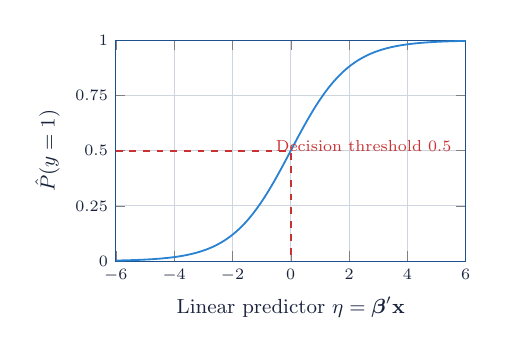
\begin{tikzpicture}[scale=0.82]
				\begin{axis}[
					xlabel={Linear predictor $\eta = \bm\beta'\mathbf{x}$},
					ylabel={$\hat P(y=1)$},
					xmin=-6, xmax=6, ymin=0, ymax=1,
					grid=major, grid style={midgray!40},
					xtick={-6,-4,-2,0,2,4,6},
					ytick={0,0.25,0.5,0.75,1},
					axis line style={navyblue},
					tick label style={font=\scriptsize, color=darktext},
					label style={font=\small, color=darktext},
					width=7cm, height=5cm
					]
					\addplot[oceanblue, thick, smooth, domain=-6:6, samples=80]
					{1/(1+exp(-x))};
					\addplot[alertred, dashed, thick]
					coordinates {(-6,0.5)(0,0.5)(0,0)};
					\node[alertred, font=\scriptsize]
					at (axis cs:2.5,0.52) {Decision threshold 0.5};
				\end{axis}
			\end{tikzpicture}
			\begin{exampleblock}{Binary outcome}
				\texttt{not\_working} $= 1$ if the user is retired, a student,
				or unemployed; $= 0$ otherwise ($\approx 25.6\%$ positive).
			\end{exampleblock}
		\end{frame}

% ── LR 2: Model Fitting ───────────────────────────────────────────────────────
\begin{frame}[fragile,allowframebreaks]{Logistic Regression --- Fitting the Model}
	\begin{lstlisting}[title={Book example (therinspark.com §4.4.1)}]
lr <- ml_logistic_regression(
  okc_train,
  not_working ~ scaled_age + sex
    + drinks + drugs + essay_length,
  reg_param         = 0.01,
  elastic_net_param = 0.0,   # ridge
  max_iter          = 100,
  standardization   = TRUE)

# Evaluate on test set
s <- ml_evaluate(lr, okc_test)
s$area_under_roc()   # AUC ~ 0.787
			\end{lstlisting}
			\begin{lstlisting}[title={Coefficient table via broom}]
library(broom)
tidy(lr) %>%
  arrange(desc(abs(estimate))) %>%
  head(8)
# term           estimate std.error
# sex_m           -0.492   0.031
# scaled_age      -0.387   0.019
# drinks_not_at..  0.341   0.055
# essay_length     0.0001  0.000008
			\end{lstlisting}
		\begin{block}{GLM for full inference output}
				\Rfun{ml\_generalized\_linear\_regression()} with
				\texttt{family = "binomial"} returns standard errors,
				$t$-statistics, $p$-values and AIC.
			\end{block}
			\begin{lstlisting}[title={Binomial GLM (therinspark.com)}]
glr <- ml_generalized_linear_regression(
  okc_train,
  not_working ~ scaled_age + sex
    + drinks + drugs,
  family = "binomial",
  link   = "logit")

tidy(glr)
# term         estimate std.error statistic p.value
# (Intercept) -1.172    0.022    -53.3    <2e-16
# scaled_age  -0.383    0.019    -20.2    <2e-16
# sex_m       -0.489    0.031    -15.8    <2e-16

confint(glr)
#              2.5%     97.5%
# scaled_age  -0.420   -0.346
# sex_m       -0.549   -0.429
			\end{lstlisting}
		\end{frame}

% ── LR 3: Parameter Interpretation ───────────────────────────────────────────
\begin{frame}[fragile,allowframebreaks]{Logistic Regression --- Interpreting Parameters}
	\begin{block}{Log-odds \& odds ratios}
				Each $\hat\beta_j$ is the change in the \textbf{log-odds} of
				$y=1$ for a one-unit increase in $x_j$, holding others fixed.
				\medskip

				Exponentiate to obtain the \textbf{odds ratio (OR)}:
				\[
				\widehat{OR}_j = e^{\hat\beta_j}
				\]
				If $\widehat{OR}_j > 1$: $x_j$ increases the odds of $y=1$.\\
				If $\widehat{OR}_j < 1$: $x_j$ decreases the odds.
			\end{block}
			\begin{block}{OkCupid example (key coefficients)}
				\footnotesize
				\begin{tabular}{lcc}
					\toprule
					\textbf{Term} & $\hat\beta$ & OR $= e^{\hat\beta}$\\
					\midrule
					\texttt{scaled\_age}   & $-0.387$ & $0.679$\\
					\texttt{sex\_m}        & $-0.492$ & $0.612$\\
					\texttt{drinks\_not\_at\_all} & $+0.341$ & $1.406$\\
					\bottomrule
				\end{tabular}
				\medskip

				Older users and men are \emph{less} likely to be \texttt{not\_working};
				non-drinkers are \emph{more} likely.
			\end{block}
		\begin{lstlisting}[title={Odds ratios \& CIs}]
# Exponentiate estimates and CIs
tidy(glr) %>%
  mutate(OR    = exp(estimate),
         OR_lo = exp(estimate -
                   1.96*std.error),
         OR_hi = exp(estimate +
                   1.96*std.error)) %>%
  select(term, OR, OR_lo, OR_hi)
# term            OR    OR_lo  OR_hi
# scaled_age     0.682  0.653  0.712
# sex_m          0.613  0.577  0.651
# drinks_not_at.. 1.406 1.262  1.568
			\end{lstlisting}
			\begin{lstlisting}[title={Coefficient plot}]
tidy(glr) %>%
  filter(term != "(Intercept)") %>%
  mutate(
    lo = estimate - 1.96*std.error,
    hi = estimate + 1.96*std.error) %>%
  ggplot(aes(x=term, y=estimate,
             ymin=lo, ymax=hi)) +
  geom_point(color="steelblue") +
  geom_errorbar(width=0.2) +
  geom_hline(yintercept=0,
             linetype="dashed") +
  coord_flip() +
  labs(title="Log-Odds Coefficients",
       y="Estimate", x="") +
  theme_minimal()
			\end{lstlisting}
		\end{frame}

% ── LR 4: Hypothesis Tests ────────────────────────────────────────────────────
\begin{frame}[fragile,allowframebreaks]{Logistic Regression --- Hypothesis Tests}
	\begin{block}{Wald test for $\beta_j$}
				Under $H_0: \beta_j = 0$:
				\[
				z_j = \frac{\hat\beta_j}{\mathrm{SE}(\hat\beta_j)}
				\xrightarrow{d} \mathcal{N}(0,1)
				\]
				Reject $H_0$ if $|z_j| > z_{\alpha/2}$ (typically 1.96).
			\end{block}
			\begin{block}{Likelihood ratio test (LRT)}
				Compare full model (deviance $D_1$) vs reduced (deviance $D_0$):
				\[
				\Lambda = D_0 - D_1 = -2(\ell_0 - \ell_1)
				\sim \chi^2_{q}
				\]
				where $q$ is the number of dropped parameters.
				LRT is preferred over Wald for small samples.
			\end{block}
			\begin{block}{Overall model fit: null deviance}
				\[
				D_{\text{null}} = -2\ell(\hat p_{\text{null}}),
				\quad
				D_{\text{model}} = -2\ell(\hat{\bm\beta})
				\]
				Large reduction $D_{\text{null}} - D_{\text{model}}$
				$\Rightarrow$ the predictors improve fit.
			\end{block}
		\begin{lstlisting}[title={Wald tests \& LRT via sparklyr}]
# Wald z-tests (from GLM tidy output)
tidy(glr) %>%
  select(term, estimate, std.error,
         statistic, p.value) %>%
  arrange(p.value)

# Likelihood ratio test: drop sex
glr_full    <- glr
glr_reduced <- ml_generalized_linear_regression(
  okc_train,
  not_working ~ scaled_age
    + drinks + drugs,
  family = "binomial",
  link   = "logit")

# Deviances from summary
dev_full <- glm_summary(glr_full)$deviance
dev_red  <- glm_summary(glr_reduced)$deviance

LRT <- dev_red - dev_full
pchisq(LRT, df = 1, lower.tail = FALSE)
# p << 0.001: sex is significant
			\end{lstlisting}
			\begin{alertblock}{Reminder}
				\Rfun{ml\_logistic\_regression()} uses maximum likelihood
				(L-BFGS solver by default).  It does \emph{not} produce
				Wald $p$-values; use \Rfun{ml\_generalized\_linear\_regression()}
				with \texttt{family = "binomial"} for inference.
			\end{alertblock}
		\end{frame}

% ── LR 5: Diagnostics & Evaluation ───────────────────────────────────────────
\begin{frame}[fragile,allowframebreaks]{Logistic Regression --- Diagnostics \& Model Evaluation}
	\begin{block}{Goodness-of-fit measures}
				\begin{tabular}{ll}
					\toprule
					\textbf{Metric} & \textbf{sparklyr function}\\
					\midrule
					AUC-ROC     & \texttt{s\$area\_under\_roc()}\\
					AUC-PR      & \texttt{s\$area\_under\_pr()}\\
					Accuracy    & \texttt{s\$accuracy()}\\
					F1 score    & \texttt{s\$weighted\_f\_measure()}\\
					Pseudo $R^2$ & $(D_{\text{null}}-D_{\text{model}})/D_{\text{null}}$ (manual)\\
					AIC         & from \texttt{glance(glr)}\\
					\bottomrule
				\end{tabular}
			\end{block}
			\begin{lstlisting}[title={ROC curve (therinspark.com §4.4.1)}]
s <- ml_evaluate(lr, okc_test)
roc <- s$roc() %>% collect()

ggplot(roc, aes(x=FPR, y=TPR)) +
  geom_line(color="steelblue",
            linewidth=1) +
  geom_abline(linetype="dashed",
              color="grey50") +
  labs(title = paste0(
       "Logistic Reg.  AUC = ",
       round(s$area_under_roc(),3)),
       x="False Positive Rate",
       y="True Positive Rate") +
  theme_minimal()
			\end{lstlisting}
		\begin{lstlisting}[title={Residual deviance diagnostics}]
# Pearson residuals via GLM
glm_summary <- function(m) {
  s <- summary(m)
  list(deviance = s$deviance,
       null_dev = s$null.deviance,
       AIC      = s$aic)
}

g <- glm_summary(glr)
g$null_dev  # null deviance
g$deviance  # residual deviance
g$AIC

# McFadden pseudo-R^2
1 - g$deviance / g$null_dev
# ~ 0.078 for the OkCupid model
			\end{lstlisting}
			\begin{lstlisting}[title={Confusion matrix at 0.5 threshold}]
preds <- ml_predict(lr, okc_test)

preds %>%
  mutate(
    pred_class = as.integer(
      prediction > 0.5)) %>%
  group_by(not_working, pred_class) %>%
  tally() %>% collect()
# not_working pred_class    n
#           0          0  9102   TN
#           0          1   901   FP
#           1          0  1721   FN
#           1          1  1276   TP
			\end{lstlisting}
			\begin{exercise}[Exercise]
				Adjust the decision threshold from 0.5 to 0.3 and compute
				the new precision and recall.  Which threshold is more
				appropriate if false negatives are costly?
			\end{exercise}
		\end{frame}

% ── LR 6: GLM Diagnostics ─────────────────────────────────────────────────────
\begin{frame}[fragile,allowframebreaks]{Logistic Regression --- Additional Diagnostics}
	\begin{block}{Pearson \& deviance residuals}
				\begin{tabular}{ll}
					\toprule
					\textbf{Type} & \textbf{Formula}\\
					\midrule
					Pearson & $r_i^P = (y_i - \hat p_i)/\sqrt{\hat p_i(1-\hat p_i)}$\\
					Deviance & $d_i = \mathrm{sign}(y_i-\hat p_i)\sqrt{2|y_i\ln\frac{y_i}{\hat p_i}|}$\\
					\bottomrule
				\end{tabular}
				\medskip

				Large absolute Pearson or deviance residuals flag
				poorly fitted observations.
			\end{block}
			\begin{block}{Hosmer--Lemeshow test}
				Groups observations into $g = 10$ deciles of predicted
				probability and compares observed vs.\ expected counts:
				\[
				H = \sum_{k=1}^{g}
				\frac{(O_{1k}-E_{1k})^2}{E_{1k}} +
				\frac{(O_{0k}-E_{0k})^2}{E_{0k}}
				\sim \chi^2_{g-2}
				\]
				Non-significant $p$-value suggests adequate fit.
			\end{block}
		\begin{lstlisting}[title={Pearson residuals via sampled data}]
# Collect a 5% sample for diagnostics
diag_df <- ml_predict(lr, okc_train) %>%
  select(not_working, prediction) %>%
  sample_frac(0.05) %>% collect()

diag_df <- diag_df %>%
  mutate(
    p_hat  = prediction,
    pearson = (not_working - p_hat) /
      sqrt(p_hat * (1 - p_hat))
  )

# Flag large residuals
diag_df %>%
  filter(abs(pearson) > 3) %>%
  nrow()
# Count of potential outliers
			\end{lstlisting}
			\begin{lstlisting}[title={Hosmer--Lemeshow test (via ResourceSelection)}]
# Run on sampled data in R
library(ResourceSelection)
hl <- hoslem.test(
  diag_df$not_working,
  diag_df$p_hat,
  g = 10)
hl$p.value
# p > 0.05 --> adequate fit
			\end{lstlisting}
			\begin{exampleblock}{Influence: Cook's distance for logistic}
				Collect a sample, fit a base-R \texttt{glm()} model, and
				use \texttt{cooks.distance()} or \texttt{influence.measures()}
				to identify influential cases.
			\end{exampleblock}
		\end{frame}

% ─────────────────────────────────────────────────────────────────────────────
% CLOSING SLIDE
% ─────────────────────────────────────────────────────────────────────────────
{
	\setbeamertemplate{footline}{}
	\begin{frame}[plain]
		\begin{tikzpicture}[remember picture, overlay]
			\fill[navyblue!12] (current page.south west)
			rectangle (current page.north east);
			\fill[navyblue!22]
			([xshift=8.5cm]current page.south west)
			rectangle (current page.north east);
			\fill[tealgreen!70]
			([xshift=8.5cm]current page.south west)
			rectangle ([xshift=8.60cm]current page.north west);

			% Left: key takeaways
			\node[navyblue, font=\bfseries\large, anchor=west]
			at (0.5, 6.3) {Key Takeaways};
			\node[darktext, font=\small, anchor=west] at (0.6, 5.65)
			{$\bullet$\;SLR with \texttt{scaled\_age}: $R^2=0.041$, RMSE$=1847$};
			\node[darktext, font=\small, anchor=west] at (0.6, 5.00)
			{$\bullet$\;MLR (age + sex + lifestyle): $R^2=0.118$, RMSE$=1758$};
			\node[darktext, font=\small, anchor=west] at (0.6, 4.35)
			{$\bullet$\;Use \texttt{ml\_gen\_lin\_regression(gaussian)} for $p$-values};
			\node[darktext, font=\small, anchor=west] at (0.6, 3.70)
			{$\bullet$\;Logistic regression AUC$\approx$0.787 on \texttt{not\_working}};
			\node[darktext, font=\small, anchor=west] at (0.6, 3.05)
			{$\bullet$\;Exponentiate log-odds $\rightarrow$ interpretable odds ratios};
			\node[darktext, font=\small, anchor=west] at (0.6, 2.40)
			{$\bullet$\;Diagnostics: residual plots, VIF, Cook's $D$, HL test};

			% Right: big text
			\node[navyblue, font=\bfseries\Huge, align=left, anchor=west]
			at (8.9, 5.8) {Regression};
			\node[navyblue, font=\bfseries\Huge, align=left, anchor=west]
			at (8.9, 5.0) {Modelling};
			\node[oceanblue, font=\bfseries\Large, align=left, anchor=west]
			at (8.9, 4.2) {at Scale};
			\draw[tealgreen, line width=1.5pt] (8.9,3.75) -- (13.3,3.75);
			\node[midgray, font=\footnotesize, align=left, anchor=west]
			at (8.9, 3.4)
			{\texttt{sparklyr} + Apache Spark MLlib};
			\node[midgray, font=\itshape\tiny, align=left, anchor=west]
			at (8.9, 0.5)
			{Luraschi, Kuo \& Ushey (2019).
				Mastering Spark with R. O'Reilly.};
			\node[tealgreen!80!darktext, font=\scriptsize, align=left, anchor=west]
			at (8.9, 0.9)
			{therinspark.com $\cdot$ spark.posit.co};
		\end{tikzpicture}
	\end{frame}
}

\end{document}
